\documentclass[aps,prd,twocolumn,superscriptaddress,nofootinbib,floatfix]{revtex4-2}
\usepackage{amsmath,amssymb,graphicx,booktabs,bm}
\usepackage[colorlinks=true,linkcolor=blue,citecolor=blue,urlcolor=blue]{hyperref}

\newcommand{\sinf}{s_\infty}
\newcommand{\bd}{\beta_d}
\newcommand{\bu}{\beta_u}
\newcommand{\dd}{\mathrm{d}}

\begin{document}

\title{The spectral index of Fermi acceleration at ultra-relativistic shocks:\\
25 digits, all dimensions, arbitrary scattering, and the breakdown of the spectrum--anisotropy identity}

\author{[Author name]}
\affiliation{[Affiliation]}

\date{\today}

\begin{abstract}
Test particles that diffuse isotropically in direction angle at an ultra-relativistic shock acquire a power-law
spectrum $f\propto p^{-s}$. For a 3D gas, published values of the limiting index span the range 4.22--4.24. The
most precise is $4.227\pm0.001$, and an analytic approximation gives $38/9$. We reduce the
$\Gamma_u\to\infty$ problem to a single Legendre operator with two weights, joined across the shock by a
power-law factor. In this limit the upstream eigenfunctions are exact Laguerre (3D) or Hermite (2D) functions.
We then solve the eigenfunction-matching condition in ball arithmetic with up to 320 modes. A model-selected
extrapolation, whose truncation error contains an $N^{-6}\log N$ term, gives
$\sinf=4.226\,978\,816\,696\,084\,932\,553\,273$ in 3D ($\beta_d=1/3$) and
$\sinf=3.298\,508\,056\,390\,718\,143\,338\,299$ in 2D ($\beta_d=1/2$; energy index $2.2985\ldots$). Both are
confirmed by an independent discrete-ordinates solver and by a finite-$\Gamma$ solver. The numbers exclude
$38/9$ in 3D and $(1+\sqrt{13})/2$ for the 2D energy index. They also show that the Keshet--Waxman
spectrum--anisotropy relation, presented as exact for isotropic diffusion, is violated: the grazing-incidence
anisotropy is $0.85950(2)$ against the required $0.83512$ (3D), and $0.70965(1)$ against $0.66532$ (2D). We trace
the violation to a non-analytic corner of the forward--backward transport problem at grazing incidence on the
shock. We further give the exact return probability $P_{\rm ret}=0.378985$ (3D), in conflict with the
Monte-Carlo value $0.437\pm0.002$, the full curve $\sinf(\beta_d)$ to ${\sim}18$ digits, its slope
$2.879467949325874$ at $\beta_d\to0$, and the leading finite-$\Gamma$ correction.

The method extends to three further settings.
(i) In $d$ spatial dimensions the upstream modes are generalized Laguerre functions $L_n^{((d-3)/2)}$. The
energy index decreases monotonically from $2.2985$ ($d=2$) to the Newtonian strong-shock value: numerically
$s_E(d)=2+2/d-7.1(1)\,d^{-3/2}+\ldots$, with the limit $2$ confirmed to $3\times10^{-8}$.
(ii) Upstream scattering drops out of the $\Gamma_u\to\infty$ limit entirely. For downstream scattering we give
the exact linear-response kernel $K(\mu)=\delta s/\delta\ln D(\mu)$. It is smooth and shows no enhanced
sensitivity at grazing incidence, and it reproduces nonperturbative results for weak anisotropy. For the tangled-field
scattering law of Kirk et al.\ we obtain $\sinf=4.2126801838$, a shift of $-0.0143$ (approximations: $-0.02$ and
$+0.03$).
(iii) For a strong shock into a cold gas with the J\"uttner--Synge equation of state, we compute $s$ at all
speeds. It falls \emph{below} the Newtonian value $4$ for $\Gamma_u\beta_u<0.9249$, reaching a minimum
$s=3.988970$ at $\Gamma_u\beta_u=0.5541$.
\end{abstract}

\maketitle

%=====================================================================
\section{Introduction}

First-order Fermi acceleration at relativistic collisionless shocks is the standard explanation for the
non-thermal electrons that radiate in gamma-ray-burst afterglows, relativistic jets and pulsar-wind nebulae.
It is also the process studied in particle-in-cell (PIC) simulations of Weibel-mediated shocks
\cite{Spitkovsky2008,SironiSpitkovskyArons2013,SironiKeshetLemoine2015}. The canonical theoretical benchmark is
the test-particle problem: an infinitely thin planar shock moving with Lorentz factor $\Gamma_u\to\infty$ into an
unmagnetized medium, with particles diffusing isotropically in direction angle on both sides. Because the
problem has no intrinsic momentum scale, the spectrum is a power law $f\propto p^{-s}$, and $s$ is a pure number
fixed by kinematics and the downstream equation of state.

That number has been computed many times:
\begin{itemize}
\item Monte-Carlo simulations gave $s\approx4.2$ \cite{BednarzOstrowski1998} and $4.22\pm0.01$
  \cite{Achterberg2001}.
\item The eigenfunction method of Kirk et al.\ (KGGA) \cite{KGGA2000}, which builds on
  \cite{KirkSchneider1987,HeavensDrury1988}, gave $4.23\pm0.01$.
\item A moment expansion gave $4.24$ at order six \cite{Keshet2006}.
\item A finite-difference relaxation code gave $4.227\pm0.001$ \cite{NagarKeshet2021}.
\item Keshet and Waxman (KW) \cite{KeshetWaxman2005} derived an identity between $s$ and the anisotropy of
  particles moving along the shock front, presented as exact for isotropic diffusion. Truncating it gave the
  closed form $s=(3\bu-2\bu\bd^2+\bd^3)/(\bu-\bd)$, hence $s=38/9$ in the ultra-relativistic limit.
\end{itemize}
In 2D, which is the geometry of most PIC studies, the analogous approximation gives an energy index
$s_E=(1+\sqrt{13})/2$ \cite{Lavi2020,NagarKeshet2021}.

In this paper we solve the benchmark problem to 25 significant digits in both 3D and 2D, and establish the
following:
\begin{enumerate}
\item The index (Sec.~\ref{sec:results}). The values exclude the closed forms above and settle the spread among
  numerical values.
\item The spectrum--anisotropy identity is not exact. It fails because the shock-front distribution is
  non-analytic at grazing incidence (Sec.~\ref{sec:kw}).
\item The exact return probability per cycle disagrees with the published Monte-Carlo value
  (Sec.~\ref{sec:pret}).
\end{enumerate}
We also give the full dependence $\sinf(\bd)$ on the downstream speed, its expansion about the infinitely
compressive limit, and the leading finite-$\Gamma$ correction. Three extensions follow:
\begin{itemize}
\item the index in any spatial dimension, and its approach to the Newtonian value (Sec.~\ref{sec:dim});
\item the exact response of $s$ to an arbitrary scattering law, including KGGA's tangled-field model
  (Sec.~\ref{sec:scat});
\item the index for physical strong shocks at all speeds (Sec.~\ref{sec:js}).
\end{itemize} The computations used the BootLoops harness
\cite{BootLoops}: Arb ball arithmetic \cite{Johansson2017} and its integer-relation gate
\cite{FergusonBaileyArno1999}.

%=====================================================================
\section{Formulation}
\label{sec:form}

We follow KGGA \cite{KGGA2000}. In each fluid's rest frame the particle has momentum $p$ and direction cosine
$\mu$ with respect to the shock normal. The distance $z$ is measured in the shock frame; the flow is along $+z$,
with the upstream at $z<0$ moving at speed $\bu$ and the downstream at $z>0$ moving at speed $\bd$. The
stationary transport equation is
\begin{equation}
\Gamma(\beta+\mu)\,\partial_z f=\partial_\mu\!\left[(1-\mu^2)D\,\partial_\mu f\right].
\label{eq:transport}
\end{equation}
Here $D$ is constant on each side (isotropic diffusion in direction angle), and $\Gamma$ and $\beta$ take their
upstream or downstream values. The boundary conditions are $f\to0$ as $z\to-\infty$ and $f$ bounded as
$z\to+\infty$. The invariant $f$ is continuous at $z=0$ under the boost
$\beta_r=(\bu-\bd)/(1-\bu\bd)$:
\begin{equation}
p_+=\Gamma_rp_-(1+\beta_r\mu_-),\qquad \mu_+=\frac{\mu_-+\beta_r}{1+\beta_r\mu_-},
\label{eq:boost}
\end{equation}
where $-$ and $+$ label the upstream and downstream frames. Separating variables gives modes
$Q(\mu)e^{\Lambda z/\Gamma}$ with
\begin{equation}
\bigl((1-\mu^2)Q'\bigr)'=\Lambda(\beta+\mu)Q ,
\label{eq:eig}
\end{equation}
with $Q$ regular at $\mu=\pm1$. Downstream, the allowed modes have $\Lambda\le0$; this includes the isotropic
mode $\Lambda=0$, which carries particles to $z=+\infty$. Upstream, the allowed modes have $\Lambda>0$. The
equation is of forward--backward type: the weight $\beta+\mu$ changes sign at the \emph{grazing} direction
$\mu=-\beta$, where particles move parallel to the shock in the shock frame.

\subsection{The limit $\Gamma_u\to\infty$}
\label{sec:limit}

Let $\varepsilon=1-\bu$ and $y=(1+\mu_-)/\varepsilon$. Then $\bu+\mu_-=\varepsilon(y-1)$,
$1-\mu_-^2=\varepsilon y(2-\varepsilon y)$, and $\partial_\mu=\varepsilon^{-1}\partial_y$, so to leading order
Eq.~\eqref{eq:eig} upstream becomes
\begin{equation}
\partial_y(2y\,\partial_y g)=\tilde\Lambda\,(y-1)\,g .
\end{equation}
Substituting $g=e^{-ay}h$ with $2a^2=\tilde\Lambda$ gives Laguerre's equation in $2ay$ with index
$n=(a-1)/2$. Solutions regular at $y=0$ and bounded as $y\to\infty$ therefore exist exactly for $a=2n+1$:
\begin{equation}
Q_n(y)=e^{-(2n+1)y}L_n\bigl((4n+2)y\bigr),\qquad \tilde\Lambda_n=2(2n+1)^2 .
\label{eq:laguerre}
\end{equation}
These are the asymptotic eigenfunctions of Kirk \& Schneider \cite{KirkSchneider1989,KGGA2000}, here obtained in
closed form. Define $\kappa=(1+\bd)/(1-\bd)$, so $\kappa=2$ for $\bd=1/3$. Then $1-\beta_r=\kappa\varepsilon+O(\varepsilon^2)$, and
Eq.~\eqref{eq:boost} becomes
\begin{equation}
\mu_+=\frac{y-\kappa}{y+\kappa},\qquad \frac{p_+}{p_-}=\sqrt{\frac{\varepsilon}{2\kappa}}\,(y+\kappa).
\end{equation}
Write $F(\mu_+)$ for the downstream-frame angular distribution at the shock, defined by $f=p_+^{-s}F$. It is
related to the upstream one, $g(y)$, by
\begin{equation}
F(\mu_+)\propto(y+\kappa)^s\,g(y)\propto(1-\mu_+)^{-s}g .
\label{eq:match}
\end{equation}
The grazing directions coincide: $\mu_+=-\bd$ if and only if $y=1$.

\paragraph{Unified form.}
Substituting $y=\kappa(1+\mu)/(1-\mu)$ gives
$\partial_y(2y\partial_y)=\frac{(1-\mu)^2}{2\kappa}\partial_\mu(1-\mu^2)\partial_\mu$ and
$y-1=(\kappa+1)(\bd+\mu)/(1-\mu)$. In the downstream variable both sides therefore obey the same operator, with
different weights:
\begin{equation}
\bigl((1-\mu^2)Q'\bigr)'=\Lambda\,w\,Q,\quad
w=\begin{cases}\bd+\mu & \text{(down)},\\[2pt] \dfrac{\bd+\mu}{(1-\mu)^{3}}&\text{(up)}.\end{cases}
\label{eq:unified}
\end{equation}
The two sides are glued by Eq.~\eqref{eq:match}. The upstream weight has an irregular singular point at
$\mu=1$, which produces the essential decay $e^{-(2n+1)y}$.

\subsection{Two dimensions}

For momenta confined to a plane with angle $\phi$ to the normal, isotropic angular diffusion replaces the right
side of Eq.~\eqref{eq:eig} by $\partial_\phi^2$, giving $Q''=\Lambda(\beta+\cos\phi)Q$ with $Q$ even. Near
$\phi=\pi$, set $\theta=\pi-\phi=(2\varepsilon)^{1/2}t$; the upstream problem becomes $Q_{tt}=\lambda(t^2-1)Q$,
a harmonic oscillator. Its even, decaying solutions with $y=t^2=(1+\mu_-)/\varepsilon$ are
\begin{equation}
Q_n(y)=e^{-(4n+1)y/2}L_n^{(-1/2)}\bigl((4n+1)y\bigr),\quad \lambda_n=(4n+1)^2 .
\end{equation}
The kinematics, Eq.~\eqref{eq:match}, are unchanged. We take $\bd=1/2$, the 2D analogue of $\bd=1/3$ (an
ultra-relativistic 2D gas has adiabatic index $3/2$).

%=====================================================================
\section{Method}
\label{sec:method}

\paragraph{Petrov--Galerkin condition.}
$F$ lies in the closed span of the downstream $\Lambda\le0$ modes if and only if it is orthogonal, in the
indefinite inner product $\langle a,b\rangle=\int(\bd+\mu)ab\,\dd\mu$, to every downstream mode with $\Lambda>0$.
This follows from the full-range orthogonality and completeness of the eigenfunctions of forward--backward
equations \cite{Beals1981,KGGA2000}. Expand $g=\sum_{n<N}a_nQ_n$ and test against the $N$ lowest downstream
$\Lambda>0$ modes $Q^+_j$ (in 2D the measure is $\dd\phi$). The condition becomes $\det S(s)=0$ with
\begin{equation}
S_{jn}(s)=\int_{-1}^{1}(\bd+\mu)\,\bigl(y(\mu)+\kappa\bigr)^s\,Q_n\bigl(y(\mu)\bigr)\,Q_j^+(\mu)\,\dd\mu .
\label{eq:S}
\end{equation}
This is KGGA's ``new method'' \cite{KGGA2000} in the limit, with exact trial functions.
\footnote{In $y$-space the integrand is $(y-1)(y+\kappa)^{s-3}Q_nQ_j^+$. Ref.~\cite{KGGA2000} prints the
factor as $(y+2)^{-s}$. Our finite-$\Gamma$ solver (Sec.~\ref{sec:valid}), which uses the exact boost
Eq.~\eqref{eq:boost}, converges to Eq.~\eqref{eq:S}.}

\paragraph{Downstream eigenpairs.}
In the orthonormal Legendre basis $\{p_k\}$, Eq.~\eqref{eq:eig} becomes the three-term recurrence
\begin{equation}
k(k+1)c_k+\Lambda\bigl(\beta c_k+b_{k-1}c_{k-1}+b_kc_{k+1}\bigr)=0,
\end{equation}
with $b_k=(k+1)/\sqrt{(2k+1)(2k+3)}$.
In 2D the cosine basis gives $k^2$ in place of $k(k+1)$, with $b_0=2^{-1/2}$ and $b_{k\ge1}=1/2$. Regularity at
both ends selects the minimal solution, computed by backward recurrence. The eigenvalues are the roots of
$\beta+b_0c_1/c_0=0$. They are seeded in double precision from the reduced symmetric tridiagonal problem and
refined by secant iteration.

\paragraph{Arithmetic and quadrature.}
All quantities are Arb balls \cite{Johansson2017} at $200+3N$ bits. The precision must grow with $N$ because the
trial basis \eqref{eq:laguerre} loses about $0.73$ digits of conditioning per mode. The integral \eqref{eq:S} is
split at $\mu=-\bd$. On $[-1,-\bd]$ we use Gauss--Legendre with $8N+120$ nodes; on $y\in[1,2^9]$ we use dyadic
Gauss--Legendre panels with 80 nodes each. The Legendre series are truncated at $6N+120$ terms. The root in $s$
is found by Newton iteration with $\dd\log\det S/\dd s=\mathrm{tr}(S^{-1}S')$.

\paragraph{Extrapolation.}
Table~\ref{tab:sN} lists $s_N$ for $N$ up to 320 (3D) and 160 (2D); Fig.~\ref{fig:conv} shows the convergence.
The local exponent tends to 4 from above. To choose the asymptotic model, we fit each candidate exactly on $m+1$
consecutive values of $N$ and predict the next, larger $N$ out of sample. The model
\begin{align}
s_N=\sinf&+aN^{-4}+bN^{-5}\nonumber\\
&+cN^{-6}\log N+\textstyle\sum_{k\ge6}d_kN^{-k}
\label{eq:model}
\end{align}
beats pure integer powers, powers of $N^{-1/3}$ and $N^{-2/3}$, and log terms at other orders. Its
out-of-sample errors are about 100 times smaller (Table~\ref{tab:model}), and its estimate of $\sinf$ changes
by less than $2\times10^{-27}$ between fit orders $m=7$ and $8$.

\begin{table}
\caption{Truncated eigenvalues $s_N$ (digits shown are exact for each $N$).}
\label{tab:sN}
\begin{ruledtabular}
\begin{tabular}{rll}
$N$ & 3D ($\bd=1/3$) & 2D ($\bd=1/2$)\\ \hline
2   & 4.227011365546354259 & 3.298517209472822393\\
4   & 4.226979904553625690 & 3.298508343664055128\\
8   & 4.226978864665305610 & 3.298508069242913564\\
16  & 4.226978819232631672 & 3.298508057071648065\\
32  & 4.226978816842089231 & 3.298508056429920311\\
64  & 4.226978816704844244 & 3.298508056393069977\\
128 & 4.226978816696621322 & 3.298508056390862158\\
256 & 4.226978816696118116 & \\
320 & 4.226978816696098497 & \\ \hline
$\infty$ & 4.226978816696084933 & 3.298508056390718143
\end{tabular}
\end{ruledtabular}
\end{table}

\begin{table}
\caption{Model selection for the 3D extrapolation ($N\le320$). ``pred.\ err.'' is the out-of-sample error when
predicting the largest $N$ from the next $m+1$ smaller values; $\sinf-4.2269788166960849325532$ is in units of
$10^{-26}$.}
\label{tab:model}
\begin{ruledtabular}
\begin{tabular}{lccc}
model & $m$ & pred.\ err. & $\sinf$ offset \\ \hline
integer powers $N^{-4,-5,\ldots}$ & 6 & $6.6\times10^{-25}$ & 34.3\\
                                   & 8 & $1.0\times10^{-25}$ & 60.2\\
powers of $N^{-1/3}$ from $N^{-4}$  & 8 & $1.2\times10^{-26}$ & 79.2\\
Eq.~\eqref{eq:model}               & 6 & $1.3\times10^{-26}$ & 72.1\\
                                   & 7 & $2.9\times10^{-27}$ & 72.6\\
                                   & 8 & $8.2\times10^{-28}$ & 72.8
\end{tabular}
\end{ruledtabular}
\end{table}

\begin{figure}
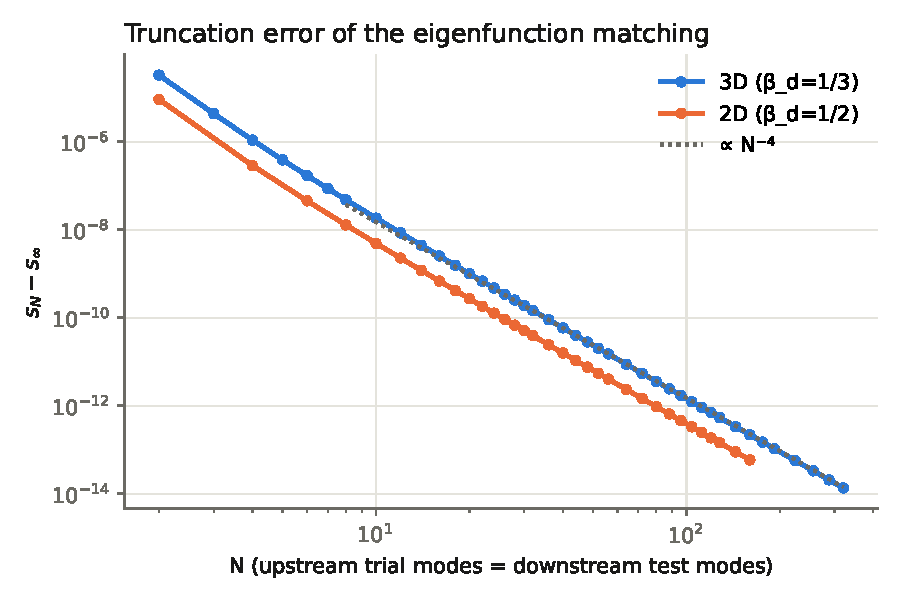
\includegraphics[width=\columnwidth]{../figures/fig2_convergence.pdf}
\caption{Truncation error $s_N-\sinf$ of the eigenfunction matching in 3D and 2D.}
\label{fig:conv}
\end{figure}

%=====================================================================
\section{Validation}
\label{sec:valid}

\begin{enumerate}
\item \emph{Discretization.} At $N=128$, the value of $s_N$ is unchanged to 50 digits when we increase the
  $y$-panel nodes ($80\to200$), the $\mu$-nodes ($1144\to1600$), the Legendre truncation ($888\to1100$), the
  $y$ cutoff, or the working precision. The out-of-sample residuals of Eq.~\eqref{eq:model}, $<10^{-27}$, bound
  any discretization noise at large $N$.
\item \emph{Independent method.} We also apply discrete ordinates to the unified form \eqref{eq:unified}. Both
  sides are collocated on the same $n$ Gauss--Legendre nodes, where the operator is exact on polynomials. The
  allowed subspaces, of dimensions $n_>$ and $n_<$ (nodes on either side of $-\bd$), sum to $n$. The index then
  solves $\det[V_d\,|\,\mathrm{diag}((1-\mu_k)^{-s})V_u]=0$. This method uses no Laguerre functions, no
  quadrature of Eq.~\eqref{eq:S}, and no projection. Its convergence is oscillatory, but it agrees with $\sinf$
  to ${\sim}10^{-11}$ for $n\le256$.
\item \emph{The limit itself.} A double-precision finite-$\Gamma$ solver computes the upstream modes from the
  full Legendre pencil at speed $\bu<1$ and uses the exact boost. At fixed $N$ it converges to the limiting
  $s_N$ as $\Gamma_u^{-2}$; extrapolation reproduces the limit to $2\times10^{-7}$.
\item \emph{Physical controls.} The finite-$\Gamma$ solver reproduces nonrelativistic diffusive shock
  acceleration, $s\to3r/(r-1)$ with corrections $O(\bu^2)$, for compression ratios $r=4$ and $2.5$. In the limit
  solver, $\sinf\to3$ as $\bd\to0$, where every particle returns.
\end{enumerate}

%=====================================================================
\section{Results}
\label{sec:results}

\subsection{The universal index}

The 3D index is
\begin{equation}
\boxed{\sinf^{\rm 3D}=4.226\,978\,816\,696\,084\,932\,553\,273}
\end{equation}
for $\bd=1/3$. The uncertainty is below one unit in the last digit, estimated from the spread of the
best-ranked extrapolations. The 2D index is
\begin{equation}
\boxed{\sinf^{\rm 2D}=3.298\,508\,056\,390\,718\,143\,338\,299}
\end{equation}
for $\bd=1/2$, corresponding to the energy index $s_E=s-1=2.298\,508\ldots$. Figure~\ref{fig:lit} compares the
3D value with the literature. It confirms $4.227\pm0.001$ \cite{NagarKeshet2021} and the cruder values. It
excludes $38/9$ (off by $4.76\times10^{-3}$). In 2D it excludes $s_E=(1+\sqrt{13})/2$ (off by
$4.27\times10^{-3}$).

\begin{figure}
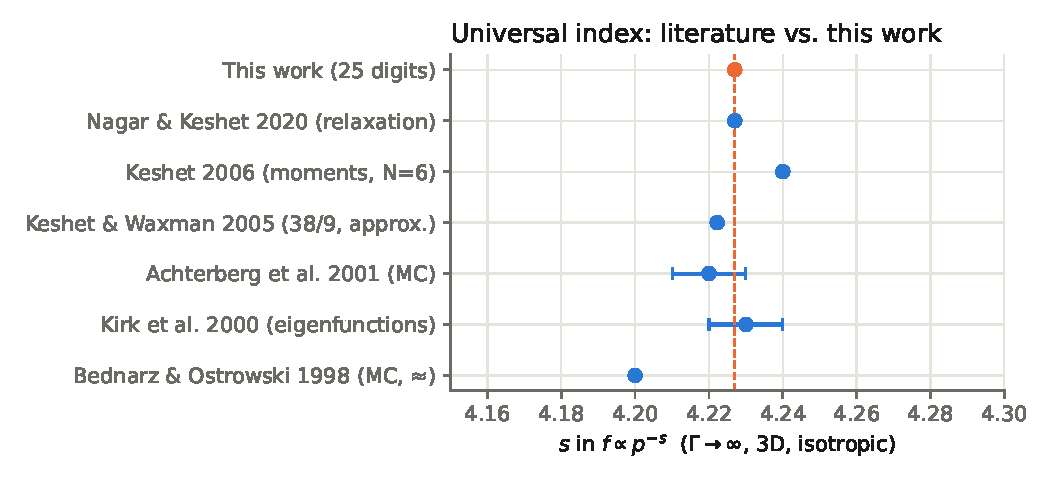
\includegraphics[width=\columnwidth]{../figures/fig1_literature.pdf}
\caption{Published values of the 3D index
\cite{BednarzOstrowski1998,KGGA2000,Achterberg2001,KeshetWaxman2005,Keshet2006,NagarKeshet2021} compared with
this work.}
\label{fig:lit}
\end{figure}

\paragraph{Closed form?}
We used BootLoops' \texttt{pslq\_gate}, which requires two-precision stability and planted positive controls
inside each basket. It finds no relation among $\{1,s,s^2,s^3\}$ with coefficients $\le10^5$. It finds none
expressing $s$ as a rational combination of $\{1,\pi,\pi^2,\log2,\log3\}$ with coefficients $\le10^3$, or of
$\{1,\sqrt2,\sqrt3,\zeta(3)\}$ with coefficients $\le10^4$. This holds for both $\sinf^{\rm 3D}$ and
$\sinf^{\rm 2D}$. At 25 digits these exclusions are necessarily weak.

\subsection{Dependence on the downstream speed}

Figure~\ref{fig:beta} and Table~\ref{tab:beta} give $\sinf(\bd)$ for $0<\bd\le0.85$, each point to
${\sim}10^{-18}$. This curve gives the $\Gamma_u\to\infty$ index for any downstream equation of state, for
example a lower compression caused by magnetization \cite{KGGA2000}, within the same scattering model. The KW
formula is accurate to $\le5.5\times10^{-3}$, but its error changes sign twice, near $\bd\simeq0.23$ and $0.55$.
Near the infinitely compressive limit,
\begin{equation}
\sinf=3+a_1\bd+a_2\bd^2+a_3\bd^3+\ldots,
\end{equation}
with $a_1=2.879\,467\,949\,325\,874$, $a_2=1.749\,393\,501\,5$ and $a_3=1.176\,62$. The KW formula instead
gives $a_1=3$.

\begin{figure}
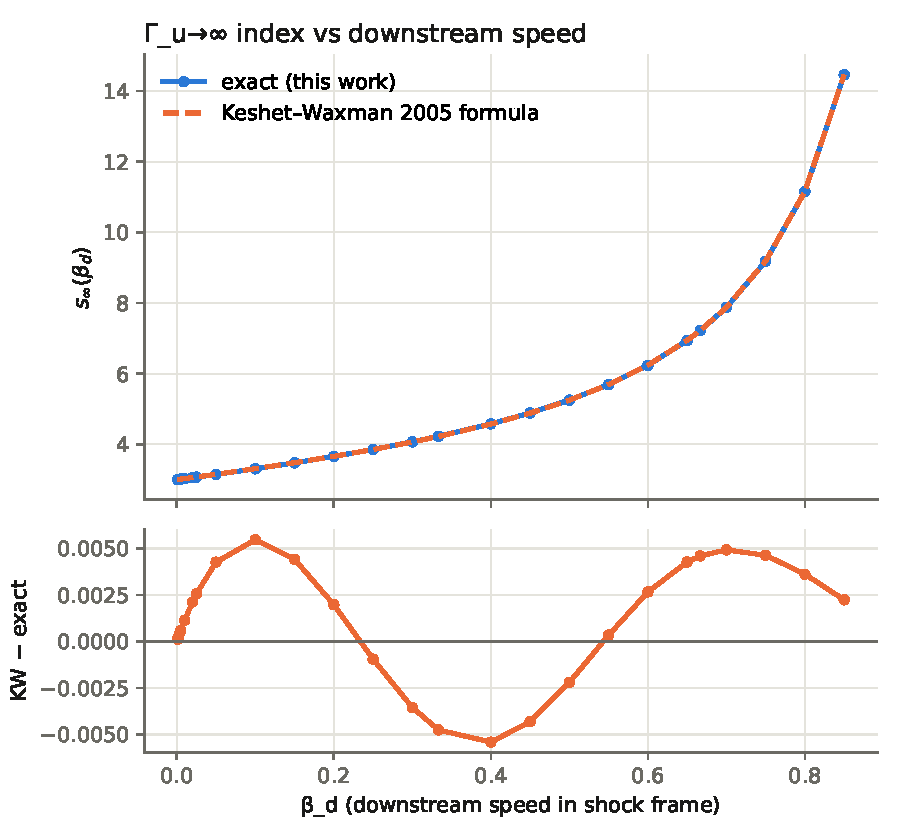
\includegraphics[width=\columnwidth]{../figures/fig3_beta_scan.pdf}
\caption{$\sinf(\bd)$ for $\Gamma_u\to\infty$ (top) and the error of the Keshet--Waxman formula (bottom).}
\label{fig:beta}
\end{figure}

\begin{table}
\caption{$\sinf(\bd)$, 3D, $\Gamma_u\to\infty$ (estimated error $\lesssim10^{-17}$), and the KW formula.}
\label{tab:beta}
\begin{ruledtabular}
\begin{tabular}{lll}
$\bd$ & $\sinf$ & KW \\ \hline
1/1000 & 3.002881218520578911 & 3.003001\\
1/100 & 3.028970806963360501 & 3.030102\\
1/10 & 3.306754917747891770 & 3.312222\\
1/5  & 3.658025754515797887 & 3.660000\\
1/4  & 3.855120826049169944 & 3.854167\\
3/10 & 4.070689184355443892 & 4.067143\\
2/5  & 4.578744853592199682 & 4.573333\\
1/2  & 5.252200597122419889 & 5.250000\\
3/5  & 6.237339907758071001 & 6.240000\\
2/3  & 7.217625960002580662 & 7.222222\\
3/4  & 9.182870847014065742 & 9.187500\\
4/5  & 11.15638644157611112 & 11.16000\\
17/20 & 14.45859724585625469 & 14.46083
\end{tabular}
\end{ruledtabular}
\end{table}

\subsection{Finite shock Lorentz factor}

At fixed $\bd=1/3$, the finite-$\Gamma$ solver gives
\begin{equation}
s(\Gamma_u)=\sinf+\frac{0.990}{\Gamma_u^2}+\frac{1.09}{\Gamma_u^4}+\ldots,
\end{equation}
a shift of $0.2\%$ at $\Gamma_u=10$. For a physical equation of state, $\bd$ itself depends on $\Gamma_u$, and
the term $(\dd\sinf/\dd\bd)\,\delta\bd$ adds to this.

%=====================================================================
\section{The spectrum--anisotropy identity}
\label{sec:kw}

KW \cite{KeshetWaxman2005} expand the distribution in each fluid frame about grazing incidence,
$f_i=[a_0^{(i)}+a_1^{(i)}x+a_2^{(i)}x^2+\ldots]p_i^{-s}$ with $x=\mu_i+\beta_i$. At $x=0$, Eq.~\eqref{eq:transport}
gives $a_2=-a_1\beta\gamma^2$ for every $z\ne0$. Taking $z\to0$ on both sides and matching $a_0$, $a_1$ and $a_2$
through Eq.~\eqref{eq:boost} yields one relation between $s$ and the downstream anisotropy
$\rho_d=a_1^{(d)}/a_0^{(d)}=F'(-\bd)/F(-\bd)$. Repeating their algebra symbolically for $\bu\to1$ reproduces
their result in 3D. It also gives the 2D analogue, in which the operator $\partial_\phi^2$ gives
$a_2=-a_1\beta\gamma^2/2$:
\begin{align}
\rho_d^{\rm 3D}&=\frac{(1-\bd)s-(1+\bd)}{2(1-\bd^2)}, \label{eq:kw3}\\
\rho_d^{\rm 2D}&=\frac{s\,[(1-\bd)s-\bd]}{(1-\bd^2)(2s+1)} . \label{eq:kw2}
\end{align}
With the exact indices, the identity requires $\rho_d=0.835117$ (3D) and $0.665318$ (2D).

We compute $F'(-\bd)/F(-\bd)$ from the Galerkin null vector and check it against finite differences. It
converges as $N^{-2/3}$ (Fig.~\ref{fig:kw}), and all extrapolation ans\"atze give
\begin{equation}
\rho_d^{\rm 3D}=0.85950\pm0.00002,\qquad \rho_d^{\rm 2D}=0.70965\pm0.00001 .
\end{equation}
These are violations of $2.9\%$ and $6.7\%$. Inserting the true anisotropies into Eqs.~\eqref{eq:kw3} and
\eqref{eq:kw2} would predict $s=4.292$ and $3.438$. The discrete-ordinates solution independently gives
$\rho_d^{\rm 3D}\simeq0.862$ at $n=48$, on the same decreasing trend. So the identity is not exact, even though
KW's closed-form approximation (which assumed $a_1^{(d)}/a_0^{(d)}=\bu-\bd/2=5/6$) happens to land within
$5\times10^{-3}$ of the true $s$.

\begin{figure*}
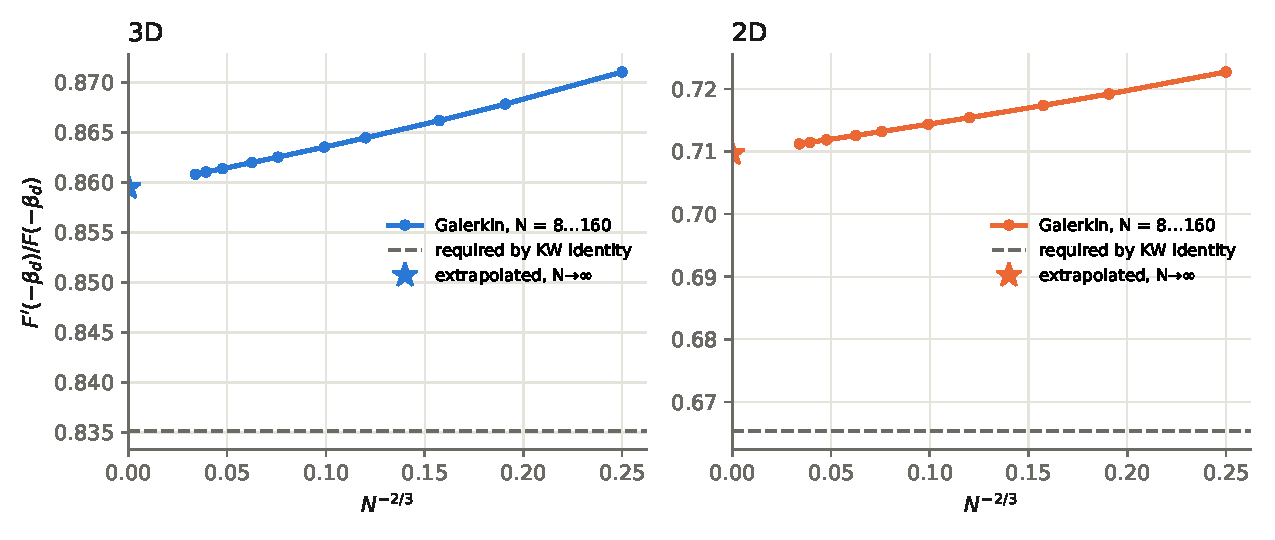
\includegraphics[width=0.75\textwidth]{../figures/fig5_kw_identity.pdf}
\caption{Grazing-incidence anisotropy $F'(-\bd)/F(-\bd)$ against $N^{-2/3}$; stars mark the extrapolated limits.
The dashed lines are the values required by Eqs.~\eqref{eq:kw3} and \eqref{eq:kw2}.}
\label{fig:kw}
\end{figure*}

\paragraph{Mechanism.}
The derivation assumes that the second-order coefficient of the \emph{trace} $F(\mu)$ equals the limit of
$a_2(z)$ as $z\to0^\pm$. Near $(z,x)=(0,0)$, both sides of the unified problem \eqref{eq:unified} reduce, after
rescaling $z$ separately on each side, to the same forward--backward equation $x\,\partial_\zeta f=\partial_x^2f$.
Write $g=(1-\mu)^s\tilde F$ upstream so that $\tilde F$ is continuous across the shock. The two sides then
differ only at sub-leading order, through a drift term ($-2s(1-\bd)\partial_x$ upstream) and the $O(x)$ variation
of the upstream weight. Under the scaling $x\sim\ell$, $\zeta\sim\ell^3$, this mismatch is smaller by one power of
$\ell$. It excites a corner solution of degree two, $\zeta^{2/3}\Phi(x/\zeta^{1/3})$. Such a solution leaves
$a_1$ continuous but gives a finite, side-dependent $a_2(0^\pm)$, different from the one-sided second derivatives
of the trace, which may contain $x^2\log|x|$. Three observations agree with this picture:
\begin{itemize}
\item the $N^{-2/3}$ convergence of $F'$, since the upstream modes resolve the grazing point on the Airy scale
  $N^{-2/3}$;
\item the $N^{-4}=(N^{-2/3})^6$ convergence of $s_N$;
\item the $N^{-6}\log N$ term selected in Eq.~\eqref{eq:model}.
\end{itemize}
A rigorous corner analysis is left for future work.

\begin{figure}
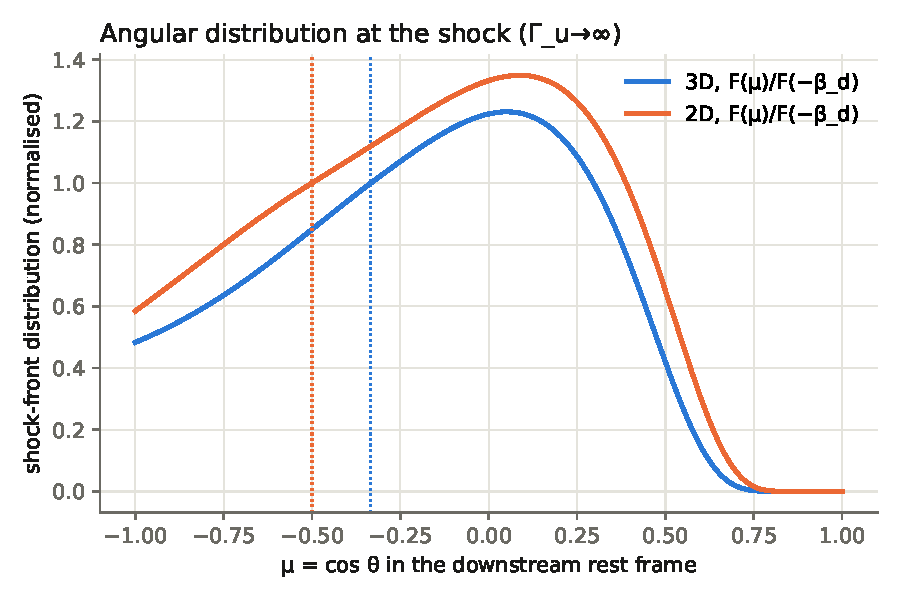
\includegraphics[width=\columnwidth]{../figures/fig4_angular.pdf}
\caption{Downstream-frame angular distribution at the shock, normalized at grazing incidence (dotted lines).}
\label{fig:ang}
\end{figure}

%=====================================================================
\section{Return probability}
\label{sec:pret}

Downstream scattering conserves $|p|$ in the downstream frame. A particle entering the downstream at momentum
$p_+$ therefore leaves, if it returns, at the same $p_+$. The return probability per cycle is then exactly the
ratio of number fluxes through the shock at fixed $p_+$:
\begin{equation}
P_{\rm ret}=\frac{\int_{-1}^{-\bd}|\bd+\mu|F\,\dd\mu}{\int_{-\bd}^{1}(\bd+\mu)F\,\dd\mu}.
\end{equation}
In 2D the measure is $\dd\phi$. We obtain $P_{\rm ret}=0.3789847$ (3D) and $0.3339262$ (2D), converged to the
digits shown; discrete ordinates give $0.37899$. Ref.~\cite{Achterberg2001} reports
$P_{\rm ret}=0.437\pm0.002$ for the same model, measured by counting each particle's downstream-to-upstream
crossings until escape, which is the same definition.

To arbitrate, we simulated the downstream half-space directly. Particles were injected with the flux-weighted
entering distribution $(\bd+\mu)F(\mu)$, $\mu>-\bd$. The direction vector performed Brownian motion on the unit
sphere with generator $D\Delta_{S^2}$, and the distance from the shock evolved as $\dot\zeta=\mu+\bd$, with an
absorbing boundary at $\zeta=12$. With $2\times10^5$ particles per run, we find $P_{\rm ret}=0.3772\pm0.0011$
($D\,\dd t=4\times10^{-3}$) and $0.3761\pm0.0011$ ($2\times10^{-3}$), and the exit-angle flux histogram matches
$|\bd+\mu|F$. This excludes $0.437$. A residual $2.9\sigma$ shortfall relative to the exact value remains at this
statistics. Its sign is the one expected from end-of-step crossing detection, which misses brief returns of
grazing particles.

The spectral index of Ref.~\cite{Achterberg2001} agrees with ours, so we suspect the discrepancy lies in the
cycle bookkeeping. We note also that the check $s=d+\ln(1/P_{\rm ret})/\ln\langle E_f/E_i\rangle$ used there is
approximate, where $d$ is the dimension. The exact steady-state condition is
$P_{\rm ret}\langle g^{\,d-s}\rangle=1$ over the distribution of energy gains $g$ per cycle. With the exact
$P_{\rm ret}$, the effective gain implied by the approximate relation is $2.2051$ (3D) and $2.3273$ (2D).

%=====================================================================
\section{Arbitrary spatial dimension}
\label{sec:dim}

Isotropic diffusion on $S^{d-1}$ acts on axisymmetric distributions through
\begin{equation}
\mathcal{L}_d=(1-\mu^2)^{-\frac{d-3}{2}}\,\partial_\mu(1-\mu^2)^{\frac{d-1}{2}}\partial_\mu ,
\end{equation}
which reduces to the operators of Sec.~\ref{sec:form} for $d=3$ and $d=2$. Its eigenfunctions are the Gegenbauer
polynomials $C_k^{(\lambda)}$, with $\lambda=(d-2)/2$ and eigenvalues $-k(k+d-2)$. They are orthogonal with
respect to $(1-\mu^2)^{\lambda-1/2}\dd\mu$. In the orthonormal basis the downstream recurrence has $k(k+d-2)$ in
place of $k(k+1)$, with
\begin{equation}
b_0=\frac{1}{\sqrt{2(\lambda+1)}},\qquad b_k=\sqrt{\frac{(k+1)(k+2\lambda)}{4(k+\lambda)(k+\lambda+1)}} .
\end{equation}
In the upstream limit $\mathcal{L}_d$ becomes $2y\partial_y^2+(d-1)\partial_y$. Repeating the reduction of
Sec.~\ref{sec:limit} gives Laguerre's equation with parameter $\alpha=(d-3)/2$. The decaying upstream modes are
\begin{equation}
Q_n(y)=e^{-a_ny}L_n^{(\frac{d-3}{2})}(2a_ny),\qquad a_n=2n+\tfrac{d-1}{2},
\label{eq:lagd}
\end{equation}
which contains Eq.~\eqref{eq:laguerre} ($d=3$) and the Hermite functions ($d=2$) as special cases. The kinematics,
Eq.~\eqref{eq:match}, do not depend on $d$.

For an ultra-relativistic $d$-dimensional gas, $p=e/d$, so $\bd=1/d$. We quote the energy index
$s_E=s-(d-1)$. For comparison, a Newtonian strong shock in a monatomic $d$-dimensional gas has compression $r=d+1$.
Its index is then $s=dr/(r-1)=d+1$, i.e.\ $s_E=2$ in every dimension.

The general-$d$ solver reproduces the $d=2$ and $d=3$ results to all 40 digits computed. At large $d$ the
truncation sequence reaches its asymptotic $N^{-4}$ regime only for $N\gtrsim\sqrt d$. We therefore scale the
$N$-range as $\max(12,\lceil\sqrt d\,\rceil)\times\{1,\ldots,4\}$; at $d=1024$ the discretization is converged to
25 digits. Table~\ref{tab:dim} and Fig.~\ref{fig:dim} give the results. For non-integer $d$ the extrapolation is
less clean: the error is $8\times10^{-11}$ at $d=5/2$, against $10^{-17}$ at integer $d$.

\begin{table}
\caption{Energy index $s_E=s-(d-1)$ for $\Gamma_u\to\infty$, $\bd=1/d$, with the extrapolation error.}
\label{tab:dim}
\begin{ruledtabular}
\begin{tabular}{rll}
$d$ & $s_E$ & error\\ \hline
2 & 2.29850805639071814 & $10^{-18}$\\
3 & 2.22697881669608492 & $10^{-17}$\\
4 & 2.18595312826943077 & $10^{-16}$\\
5 & 2.15886819749245212 & $10^{-16}$\\
6 & 2.13944467064007694 & $10^{-16}$\\
8 & 2.11313234124007319 & $10^{-15}$\\
10 & 2.09591143426758012 & $10^{-15}$\\
16 & 2.06713513896664777 & $10^{-14}$\\
32 & 2.03876545233014850 & $10^{-13}$\\
64 & 2.02178264132778 & $10^{-12}$\\
128 & 2.0119405751088 & $10^{-10}$\\
256 & 2.0064086029238 & $10^{-10}$\\
512 & 2.0033806330794 & $10^{-9}$\\
1024 & 2.00175910792 & $10^{-8}$
\end{tabular}
\end{ruledtabular}
\end{table}

\begin{figure*}
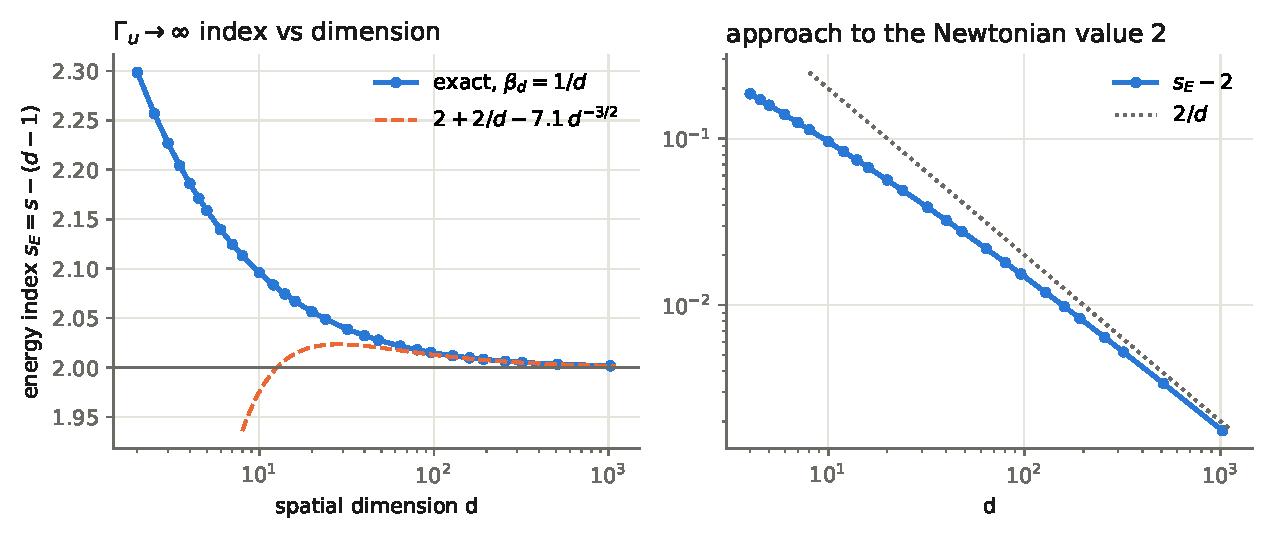
\includegraphics[width=0.8\textwidth]{../figures/fig6_dimension.pdf}
\caption{Left: energy index versus dimension, with the large-$d$ form \eqref{eq:larged}. Right: $s_E-2$ against
$2/d$.}
\label{fig:dim}
\end{figure*}

\paragraph{Large $d$.}
We fit $s_E(d)$ for $d\ge16$ by weighted least squares. A series in $d^{-1/2}$ fits about $10^3$ times better
than a series in $1/d$ (maximum residual $1.7\times10^{-8}$ versus $1.9\times10^{-5}$). Leaving the constant
free, the constant term converges to $2.00000003$ as terms are added; the coefficient of $d^{-1/2}$ is consistent
with zero; and the coefficient of $1/d$ converges to $2.000$ to within $2\times10^{-4}$. Hence
\begin{equation}
s_E(d)=2+\frac{2}{d}+\frac{c_{3/2}}{d^{3/2}}+O(d^{-2}),\qquad c_{3/2}=-7.1\pm0.1 .
\label{eq:larged}
\end{equation}
The ultra-relativistic index thus approaches the Newtonian strong-shock value from above, with a relativistic
excess $2/d$.

A scaling argument shows why the limit is finite and why the series runs in half-integer powers. Set
$\mu=x/\sqrt d$. Then $\mathcal{L}_d=d\,(\partial_x^2-x\partial_x)+O(1)$, an Ornstein--Uhlenbeck operator, and
the grazing point $-\bd=-1/d$ maps to $x=-d^{-1/2}\to0$. Near grazing, $y-1\simeq2x/\sqrt d$, so the kinematic
factor $(y+\kappa)^s$ with $s\simeq d$ grows like $e^{x\sqrt d}$. This cancels exactly against the upstream decay
$e^{-a_ny}$ with $a_n\simeq d/2$. What remains is a $d$-independent limiting problem, perturbed in powers of
$d^{-1/2}$. We have not attempted the perturbative computation of $c_1=2$ or $c_{3/2}$; it is a natural target.

%=====================================================================
\section{Arbitrary scattering}
\label{sec:scat}

\paragraph{Upstream scattering drops out.}
Let the upstream angular diffusion be $D_u(\mu)$, continuous and positive at $\mu=-1$. With
$\mu_-=-1+\varepsilon y$, the upstream operator becomes
$\varepsilon^{-1}\partial_y[2yD_u(-1)\partial_y]+O(1)$. The constant $D_u(-1)$ only rescales $z$, so the trial
functions \eqref{eq:laguerre} and \eqref{eq:lagd} are exact for \emph{every} upstream scattering law. KGGA noted
that the upstream $D$ matters only near $\mu=-1$ \cite{KGGA2000}; in the limit it does not matter at all.
Hence $\sinf$ is a functional of the downstream $D(\mu)$ alone.

\paragraph{General downstream scattering.}
For general $D(\mu)$, Eq.~\eqref{eq:eig} becomes $\partial_\mu[(1-\mu^2)D\,\partial_\mu Q]=\Lambda(\bd+\mu)Q$. We
solve it by Galerkin projection in the orthonormal Legendre basis. The stiffness matrix
$\int(1-\mu^2)Dp_k'p_l'\,\dd\mu$ is computed by Gauss--Legendre quadrature. The mass matrix $\bd+J$ is exact and
tridiagonal. We eliminate $c_0$ and compute the reduced pencil's eigenvectors at high precision in Arb. The
isotropic case is reproduced to all digits. For $D=(\mu^2+0.01)^{-1/2}$, doubling the Legendre size from 256 to 400
changes $s_{16}$ only in the 28th digit.

\paragraph{Linear-response kernel.}
About isotropic scattering ($d=3$, $\bd=1/3$), define
\begin{equation}
\delta\sinf=\int_{-1}^{1}K(\mu)\,\delta\ln D(\mu)\,\dd\mu .
\end{equation}
We compute $K$ by central differences, using Gaussian bumps of width $\sigma=0.03$ at 61 centres; the spacing is
$0.01$ near grazing incidence. Three checks support the result:
\begin{itemize}
\item \emph{Convergence in $N$.} At four test points, including grazing incidence, the kernel at $N=24$ agrees with $N=16$ to $1.5\times10^{-6}$.
\item \emph{Scale invariance.} Rescaling $D$ uniformly leaves $s$ unchanged, so $\int K\,\dd\mu=0$. The computed
  kernel satisfies this to $10^{-4}$, the level of its smoothing and grid error.
\item \emph{Nonperturbative test.} Applied to the tangled-field family below, $\int K\,\delta\ln D$ reproduces the
  exact shifts to $0.5\%$ ($a=10$) and $0.1\%$ ($a=3$). The deviation then grows smoothly with the anisotropy:
  $0.9\%$, $5\%$ and $17\%$ for $a=2$, $1$ and $0.5$.
\end{itemize}
The kernel (Fig.~\ref{fig:scat}) is smooth and broad. It is negative for $\mu\lesssim0.05$ (minimum $-0.32$ at
$\mu\simeq-0.40$) and positive above (maximum $+0.39$ at $\mu\simeq0.44$). So faster scattering of particles
moving back toward the shock hardens the spectrum, and faster scattering of particles receding downstream softens
it. Nothing special happens at grazing incidence: $K$ varies by less than $10^{-2}$ across $\mu=-1/3\pm0.02$, with
second differences consistent with a smooth function. A point-like dependence on $D'(-\bd)$ would add $c\,\delta'(\mu+\bd)$ to $K$. Fitting the
smoothed kernel on $-0.48<\mu<-0.18$ with a polynomial background of degree 3--5 plus this template gives $c$
consistent with zero at the $10^{-8}$ level, so $|c|<10^{-7}$. This contradicts the expectation, drawn from the
spectrum--anisotropy relation \cite{KeshetWaxman2005}, that $s$ is particularly sensitive to the derivative of $D$
for particles moving along the shock front.

\paragraph{Tangled fields.}
For KGGA's model of a field tangled on short scales along the normal, $D\propto(\mu^2+a^2)^{-1/2}$
\cite{KGGA2000}, Table~\ref{tab:aniso} gives $\sinf(a)$. At $a=0.1$, the case KGGA studied,
$\sinf=4.2126801838$, a shift of $-0.0143$ from isotropic. KGGA estimated a decrease of ``about $0.02$''. KW's
approximation for anisotropic diffusion gives $4.26$ \cite{KeshetWaxman2005}, which has the wrong sign. The index
decreases monotonically as $a\to0$, to $4.2115$ at $a=0.05$.

\begin{table}
\caption{$\sinf$ for $D\propto(\mu^2+a^2)^{-1/2}$ downstream (any upstream $D$), 3D, $\bd=1/3$.}
\label{tab:aniso}
\begin{ruledtabular}
\begin{tabular}{lll}
$a$ & $\sinf$ & error \\ \hline
0.05 & 4.2115053403 & $3\times10^{-11}$\\
0.1 & 4.2126801838 & $3\times10^{-11}$\\
0.2 & 4.21536621378 & $5\times10^{-12}$\\
0.3 & 4.217831856689 & $6\times10^{-13}$\\
0.5 & 4.22136017681089 & $3\times10^{-14}$\\
1 & 4.22493766179950 & $5\times10^{-15}$\\
2 & 4.22640358332686 & $2\times10^{-15}$\\
3 & 4.22671717421733 & $1\times10^{-15}$\\
10 & 4.22695486792644 & $1\times10^{-15}$\\
$\infty$ & 4.22697881669608 & (isotropic)
\end{tabular}
\end{ruledtabular}
\end{table}

\begin{figure*}
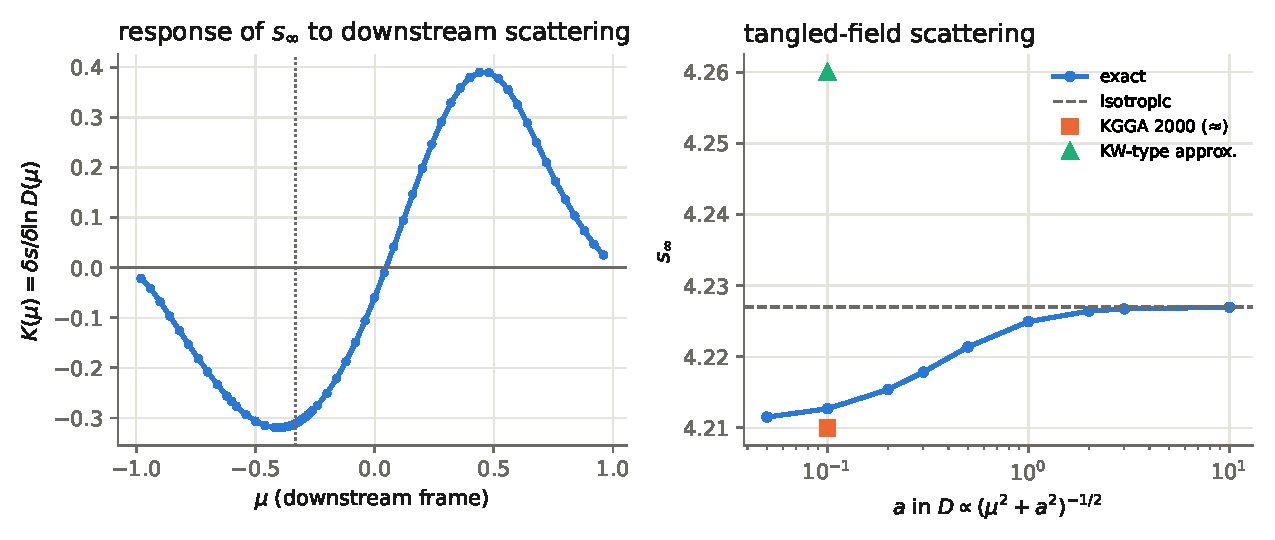
\includegraphics[width=0.8\textwidth]{../figures/fig7_scattering.pdf}
\caption{Left: linear-response kernel of $\sinf$ to the downstream scattering profile (smoothed on scale
$\sigma=0.03$; the dotted line marks grazing incidence). Right: $\sinf$ for tangled-field scattering, with the
previous estimates at $a=0.1$.}
\label{fig:scat}
\end{figure*}

%=====================================================================
\section{Physical strong shocks at all speeds}
\label{sec:js}

Consider a strong shock into a cold gas ($w_u=1$, $p_u=0$) whose downstream state is a J\"uttner--Synge gas at
temperature $\theta=kT/mc^2$, with specific enthalpy $w=K_3(1/\theta)/K_2(1/\theta)$ and $p/\rho=\theta$. The
jump conditions close in closed form:
\begin{itemize}
\item energy per particle in the downstream frame equals the relative Lorentz factor, $\Gamma_r=w-\theta$;
\item the Taub adiabat, $w^2-1=\theta(R+w)$, gives the compression $R=\rho_d/\rho_u=(w^2-1-\theta w)/\theta$;
\item mass flux, $\Gamma_u\bu=R\,\Gamma_d\bd$, then fixes $(\bu,\bd)$.
\end{itemize}
These reproduce $R\to4$ nonrelativistically, and $R\to4\Gamma_r$ with $\bd\to1/3$ in the ultra-relativistic limit.

We compute $s$ with the finite-$\Gamma$ solver, extrapolating $N\in\{8,12,16,20\}$. The accuracy is about
$10^{-9}$ for $\Gamma_u\bu\le10$, degrading to $10^{-7}$ and $10^{-6}$ at $\Gamma_u\bu=19$ and $35$ because of
double precision. Table~\ref{tab:js} and Fig.~\ref{fig:js} give the results. The index is not monotonic. It
falls below the Newtonian value 4 and reaches a minimum
\begin{equation}
s_{\min}=3.988970\quad\text{at}\quad\Gamma_u\bu=0.5541,
\end{equation}
where $\bu=0.4847$, $\theta=0.0518$ and $R=4.398$.
At the minimum, $\bd=0.1250003$, close to but measurably distinct from $1/8$. The index returns to $s=4$ at
$\Gamma_u\bu=0.9249$ ($\bu=0.6790$, $R=4.995$) and then rises toward $\sinf$.

The dip arises from two competing effects. The downstream gas becomes mildly relativistic ($\theta\sim0.05$), so
its compression rises above 4; the nonrelativistic formula $3R/(R-1)$ would give $3.88$ at the minimum. The
anisotropy that sets in at these speeds partly offsets the harder spectrum this would produce.

\begin{table}
\caption{Index for a strong shock into cold gas, J\"uttner--Synge downstream (3D isotropic scattering).}
\label{tab:js}
\begin{ruledtabular}
\begin{tabular}{lllll}
$\theta$ & $\Gamma_u\bu$ & $\bd$ & $R$ & $s$ \\ \hline
0.001  & 0.0731 & 0.01824 & 4.0075 & 3.999515259\\
0.0110 & 0.2455 & 0.06002 & 4.0833 & 3.995405458\\
0.0367 & 0.4595 & 0.10674 & 4.2804 & 3.989734864\\
0.0518 & 0.5541 & 0.12500 & 4.3984 & 3.988969566\\
0.0669 & 0.6394 & 0.14011 & 4.5183 & 3.989614221\\
0.122  & 0.9099 & 0.18017 & 4.9678 & 3.999206186\\
0.223  & 1.3423 & 0.22424 & 5.8338 & 4.027235212\\
0.406  & 2.0834 & 0.26639 & 7.5383 & 4.076899320\\
0.740  & 3.4267 & 0.29918 & 10.929 & 4.136360557\\
1.35   & 5.9226 & 0.31891 & 17.602 & 4.183990476\\
2.46   & 10.556 & 0.32810 & 30.393 & 4.210297750\\
4.48   & 19.088 & 0.33161 & 54.305 & 4.2212949\\
8.17   & 34.705 & 0.33279 & 98.341 & 4.225169\\
$\infty$ & $\infty$ & 1/3 & $\infty$ & 4.226978817
\end{tabular}
\end{ruledtabular}
\end{table}

\begin{figure}
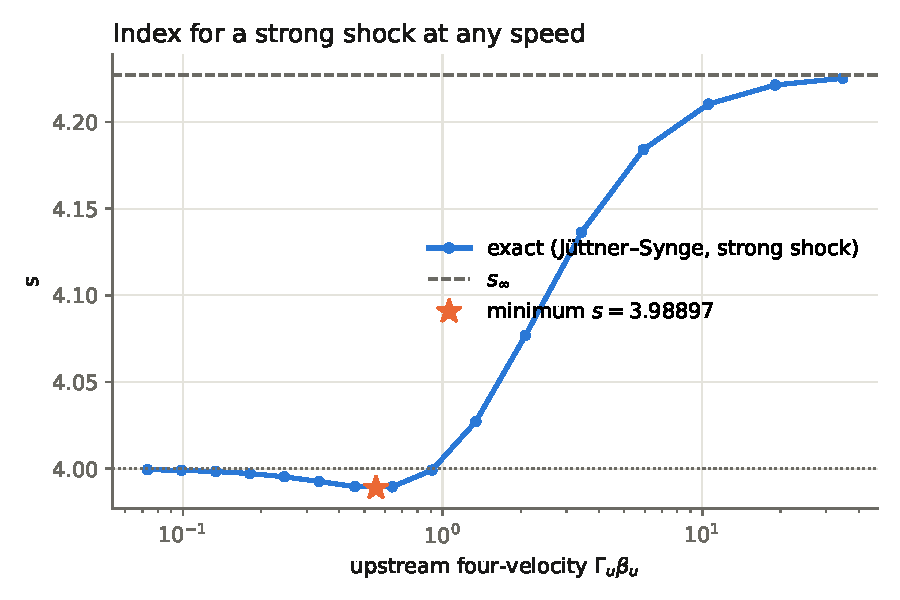
\includegraphics[width=\columnwidth]{../figures/fig8_realistic.pdf}
\caption{Spectral index of a strong shock into cold gas (J\"uttner--Synge downstream) versus upstream
four-velocity. The star marks the sub-Newtonian minimum.}
\label{fig:js}
\end{figure}

%=====================================================================
\section{Discussion}

The test-particle, isotropic-scattering, $\Gamma_u\to\infty$ index is a benchmark, not a prediction for any
particular shock. Self-generated Weibel turbulence makes scattering anisotropic and energy dependent, and the
index depends on the angular form of $D$ \cite{KGGA2000,NagarKeshet2021}. Within the benchmark, however, the
results here are definitive:
\begin{itemize}
\item They fix the reference value to 25 digits.
\item They show that two analytic shortcuts (the 38/9 and $(1+\sqrt{13})/2$ closed forms, and the
  spectrum--anisotropy identity behind them) are approximations.
\item They identify the grazing-incidence corner of the forward--backward problem as the reason those shortcuts
  fail and as the factor that controls the convergence of every angular expansion.
\end{itemize}
The same corner is the likely reason earlier moment and eigenfunction expansions stalled at a few digits. Numerical work
that uses the anisotropy identity as a consistency check \cite{KeshetWaxman2005} should treat it as approximate,
at the few-percent level in $\rho_d$. The same machinery gives:
\begin{itemize}
\item the index in any dimension, with a numerically established approach $s_E=2+2/d+\ldots$ to the Newtonian value;
\item a scattering-response kernel that turns a measured downstream $D(\mu)$, e.g.\ from PIC simulations, directly
  into a predicted index;
\item reference values for physical strong shocks at all speeds, including a
  sub-Newtonian dip.
\end{itemize}
Natural next steps are a rigorous local analysis of the corner, a perturbative derivation of the $2/d$ and
$d^{-3/2}$ coefficients, and oblique magnetized shocks.

The numerical value rests on an extrapolation in $N$ that is well tested (model selection, independent
discretizations, a finite-$\Gamma$ limit check) but not rigorous. The Arb radii certify each finite-$N$ value,
not the limit.

\begin{acknowledgments}
Computations used the BootLoops 1.0 harness \cite{BootLoops}, python-flint/Arb \cite{Johansson2017}, mpmath
\cite{mpmath}, NumPy and SciPy, run on a NERSC login node. [Disclosure to be edited by the author: the analysis code
and a first draft of this manuscript were produced with the assistance of an AI model (Claude, Anthropic).]
\end{acknowledgments}

\appendix
\section{Reproducibility}
All code and data are in the accompanying directory: \texttt{src/urnd.py} (Galerkin, 3D/2D),
\texttt{src/dord\_hp.py} (discrete ordinates), \texttt{src/finite\_gamma.py}, \texttt{src/model\_select.py},
\texttt{src/anisotropy.py}, \texttt{src/kw\_identity.py} (symbolic re-derivation of
Eqs.~\eqref{eq:kw3}--\eqref{eq:kw2}), \texttt{src/return\_prob.py}, \texttt{src/mc\_downstream.py},
\texttt{src/scan\_beta.py}; for the extensions \texttt{src/urd.py} and \texttt{src/scan\_d.py} (dimension $d$),
\texttt{src/aniso.py}, \texttt{src/kernel.py} and \texttt{src/scan\_aniso.py} (general scattering), and
\texttt{src/js\_curve.py} and \texttt{src/js\_min.py} (J\"uttner--Synge shocks); results in \texttt{results/*.json}. A single 3D value $s_{64}$ takes about 6\,s; $s_{320}$
takes about an hour on one core.

\bibliography{refs}

\end{document}
